\chapter{Implementación de algoritmos de detección y sincronismo en SDR}
\label{Ch:5}
\graphicspath{{figs/}}

En los Capítulo \ref{Ch:3} y \ref{Ch:4} se detallaron de forma independiente los algoritmos de sincronismo y detección, respectivamente, aplicables a señales que emplean OFDM en el estándar IEEE 802.11. En este capítulo se detallará la integración de dichos algoritmos en un sistema desarrollado en LabVIEW capaz de operar de forma contínua, con la función de detectar la presencia de señales transmitidas de acuerdo al estándar en las muestras adquiridas por un receptor y estimar los parámetros de sincronismo correspondientes a cada señal detectada. 

El desarrollo del sistema a diseñar contempló varias etapas. En la primera etapa se implementó un entorno de simulación del problema sobre el cual se verificó el funcionamiento del mismo con señales generadas internamente consistentes con las suposiciones hechas durante las derivaciones de los algoritmos correspondientes. En la siguiente etapa se evaluó la factibilidad de utilizar el sistema diseñado sobre señales reales adquiridas por un dispositivo periférico de radio universal programable del fabricante National Instruments NI USRP-2953R, utilizando la USRP únicamente para adquisición de muestras y realizando el procesamiento en el \textit{host}. Finalmente, se analizaron las limitaciones de este método y se consideró la necesidad de transferir una o más etapas de procesamiento a la USRP por medio del diseño de componentes FPGA personalizados.

\section{Diseño general del sistema}
\label{S:ch5-general}

\begin{figure}[t]
    \centering{}\includegraphics[width=\imsizeL]{xpstopdf/top_level.pdf}
    \caption{Diagrama de bloques \textit{top-level} del sistema que integra los algoritmos de detección y sincronismo en ejecución contínua sobre las muestras de una señal recibida implementado en LabVIEW, utilizando una simulación del problema como fuente de muestras.\label{fig:top-level-lv}}  
\end{figure}

La implementación de los algoritmos de detección y sincronismo en LabVIEW contempla una etapa de inicialización seguida de un ciclo \textit{while} que se ejecutará contínuamente. En cada iteración del ciclo \textit{while} se toma una muestra proveniente de una fuente y se registra en memoria, luego se ejecutan varias etapas secuenciales de procesamiento, y finalmente se actualiza un registro de detecciones y sus correspondientes estimaciones referentes al sincronismo. La esquemática \textit{top-level} del diseño se presenta en la Figura \ref{fig:top-level-lv}.

En un entorno de simulación, la tasa de iteraciones del ciclo \textit{while} puede ser arbitraria, pero para que el diseño implementado sea capaz de operar en tiempo real la tasa de iteraciones debe ser igual a la tasa de muestreo que tendrá el receptor. La tasa de muestreo depende del espaciamiento entre canales por medio del parámetro $T_{SHORT}$ y del número de puntos que se usarán en la FFT de recepción. En el caso típico de espaciamiento entre canales de 20 MHz y módulos FFT de 64 muestras la frecuencia de muestreo es de 20 MHz, la implementación se diseña tal que estos valores sean parametrizables.

\subsection{Etapa de inicialización}

Durante la etapa de inicialización se definen los argumentos de los algoritmos implementados que no necesitan ser calculados en cada iteración, éstos siendo la tasa de muestreo, la forma de la secuencia de entrenamiento de símbolos cortos, y las referencias que utilizará el banco de correladores. El tiempo de muestreo y la forma de la secuencia de entrenamiento de símbolos cortos depende de los valores $N_{FFT}$ y $T_{SHORT}$, mientras que las referencias dependen también del número de posibles desvíos en frecuencia de portadora utilizados y el rango de valores que se contemplan. Por este motivo, los parámetros en cuestión se necesitan definir previamente y no pueden modificarse durante la ejecución. 

\subsection{Fuente de muestras}

La fuente de muestras entrega la muestra más recientemente adquirida en banda base de una señal recibida. En el entorno de simulación estas provienen de un generador aleatorio implementado que simula un proceso Poisson con tasa de ocurrencias parametrizable al cual se le puede agregar ruido normal complejo y rotación lineal en fase proveniente de un error en frecuencia de portadora. La tasa de ocurrencias del generador, la varianza del ruido, y el error en frecuencia de portadora se pueden modificar durante la simulación.

Al momento de implementar el diseño utilizando la USRP como adquisidor, el generador Poisson se remplaza por la salida de la interfaz Rx de la librería NI-USRP provista por LabVIEW, y el resto del diseño no requeriría modificaciones.

\subsection{Registros de memoria}

La implementación de los algoritmos requiere almacenamiento de los datos entrantes y ciertos resultados intermedios en registros de memoria. Los registros utilizados son del tipo FIFO cíclica, los cuales comparten la longitud de $N$ muestras. Estos son accedidos para la escritura de un valor por un puntero de acceso $k$, el cual necesita ser un número entero módulo $N$. Los registros admiten con una señal de \textit{reset} la cual asigna 0 a todos los elementos. El diseño requiere instanciar cuatro registros de memoria, los cuales son:
\begin{itemize}
    \item $\mathbf{y}$, las muestras más recientes de la señal recibida;
    \item $\overline{\Phi}_{BC}$ y $\Phi_{DC}$, los resultados de los estadísticos del banco de correladores y el método \textit{delay and correlate} respectivamente;
    \item $\mathbf{T}$, los valores del umbral de decisión en base a las estimaciones del ruido.
\end{itemize}

El criterio con el cual se elige $N$ es tal que $\textit{y}$ sea suficientemente largo para almacenar el preámbulo de una señal entrante más un tiempo adicional de tolerancia para la detección, pero lo suficiénte corto para que no existan dos señales entrantes almacenadas simultáneamente, ya que esto produciría ambigüedad en los algoritmos de detección y sincronismo.

La necesidad de acceder a los registros por medio de un puntero en módulo $N$ implica que es conveniente expresar el índice de la iteración actual $i$ en forma de división entera más resto de división,
\begin{equation}
    i = Nc+k \qquad \text{con} \qquad c = \lfloor i/N \rfloor, \qquad k = i \bmod N.
\end{equation}

\subsection{Ventana de evaluación}

\begin{figure}[t]
    \centering{}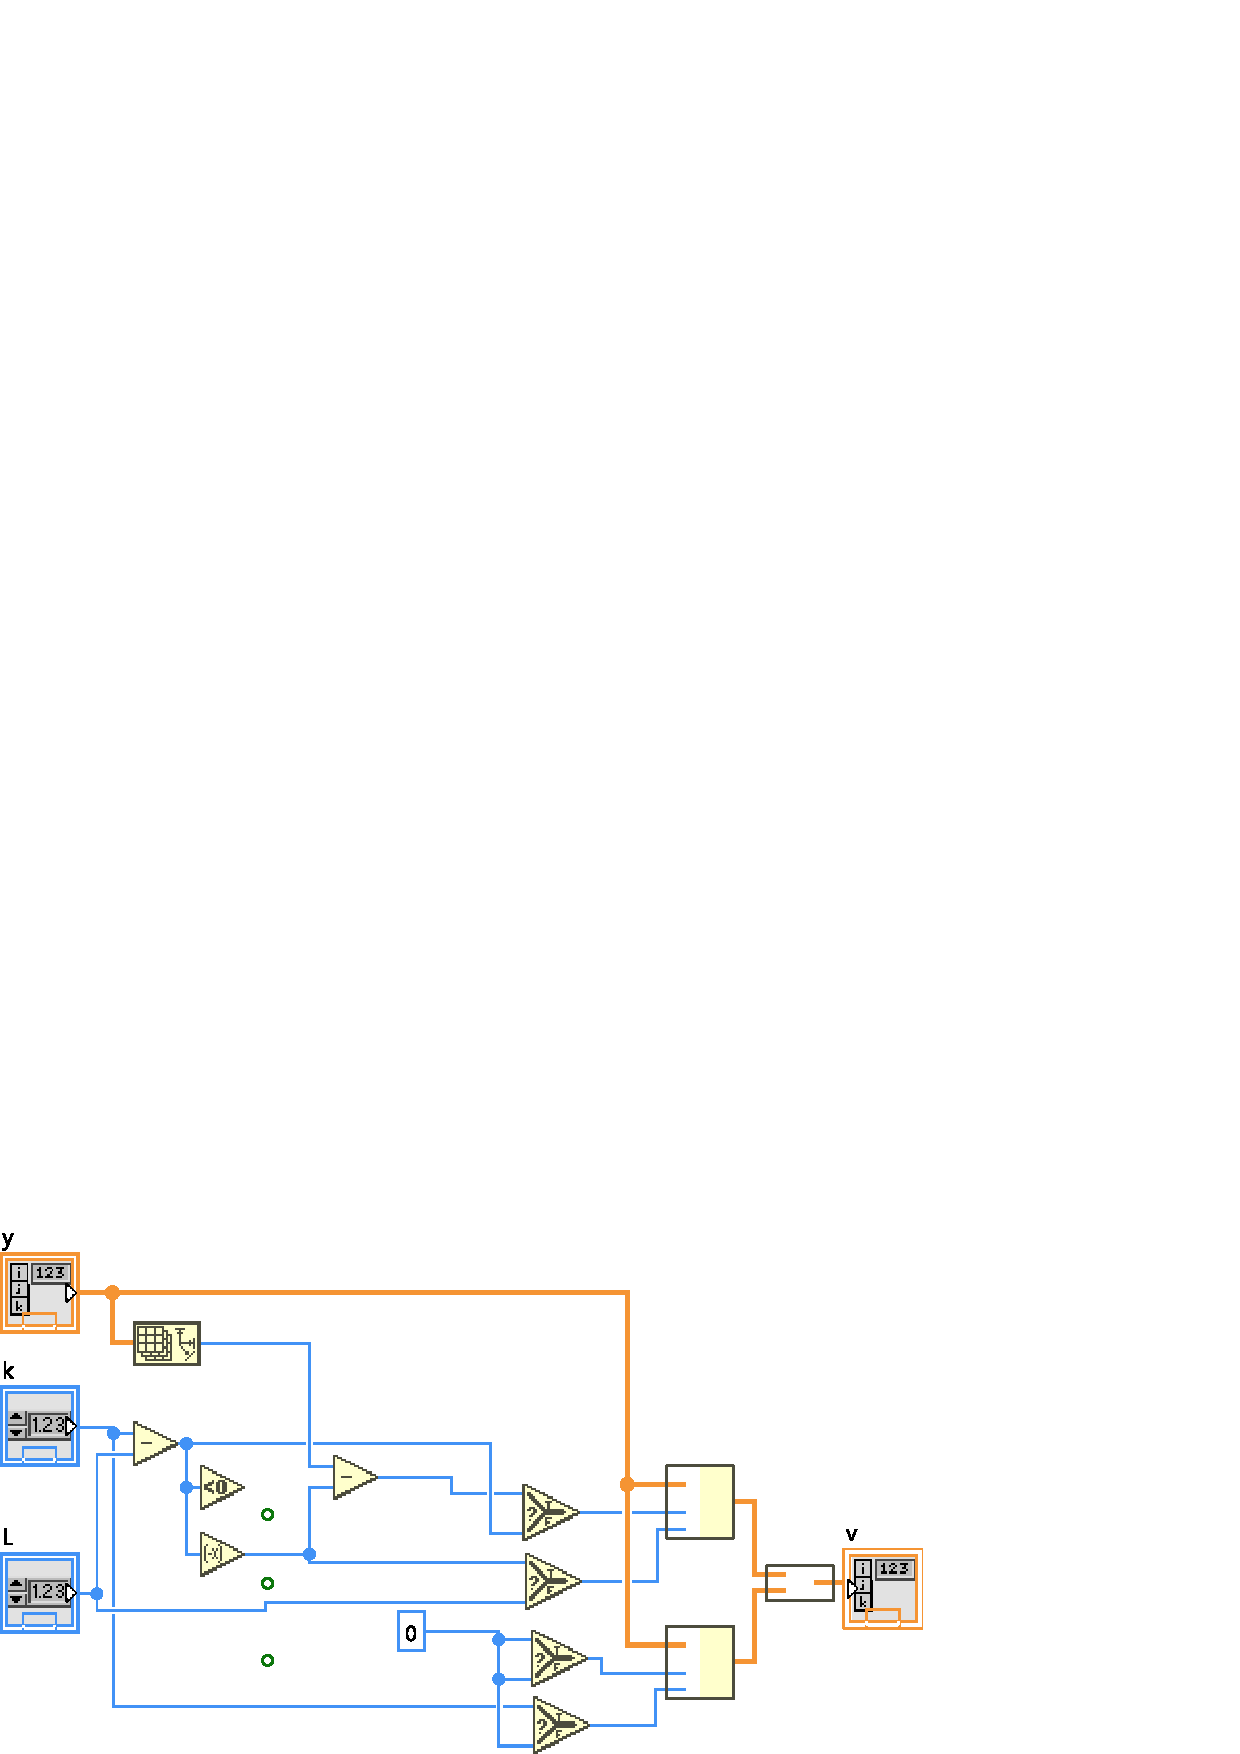
\includegraphics[width=\imsize]{xpstopdf/window.pdf}
    \caption{Diagrama de bloques de la implementación en LabVIEW del módulo que construye una ventana de evaluación $\mathbf{v}$ conteniendo las últimas $L$ muestras registradas en una FIFO cíclica $\mathbf{y}$ a partir del puntero de lectura $k$.\label{fig:window-select-lv}}  
\end{figure}

Las lecturas realizadas sobre $\mathbf{y}$ son por medio de una ventana deslizante, la cual recibe el nombre $\mathbf{v}$. Esta ventana accede a las últimas $N$ muestras registradas en determinado ciclo de iteración, de ser necesario concatenando muestras al final del registro a muestras al inicio del mismo. La asignación de los valores a $\mathbf{v}$ respecto a un puntero de iteración $k$ es la siguiente
\begin{equation}
    \mathbf{v} = \begin{bmatrix}
        y\left[(k-N+1) \bmod L\right], & \cdots, &  y\left[(k-1) \bmod L\right], & y[k]
    \end{bmatrix},
\end{equation}
en donde la longitud de la ventana $L$ es la longitud de la secuencia de entrenamiento de símbolos cortos. En la Figura \ref{fig:window-select-lv} se presenta la esquemática de la implementación en LabVIEW de ésta operación. 

En cada iteración se accede simultáneamente a $\mathbf{y}$ por dos ventanas de evaluación. La primera de estas ventanas es referenciada al instante actual $k$, y se utiliza para calcular los estadísticos $\overline{\Phi}_{BC}$ y $\Phi_{DC}$. La segunda de estas ventanas es referenciada a un ínstante anterior,
\begin{equation}
    k' = (k-2L) \bmod N,
\end{equation}
y se emplea para la estimación del ruido. El desfasaje elegido entre las ventanas es igual al doble de la longitud de la ventana ya que este asegura que ninguna de las muestras utilizadas para estimar el ruido coincida con ninguna de las muestras utilizadas para calcular los estadísticos.


\section{Estrategia de detección}
\label{S:ch5-detección}

El algoritmo de detección consiste en comparar los valores registrados del estadístico de detección con los correspondientes valores registrados del umbral. El registro del estadístico de detección recibirá el nombre de $\upphi$, y este se obtiene de tomar la fila central del registro $\overline{\Phi}_{BC}$. Sin embargo, existen ciertas consideraciones que se deben tomar en un diseño que opera en línea en cuenta para evitar ambugüedad en la detección.

El estadístico de detección produce máximos locales cuando existe presencia parcial de la secuencia de entrenamiento de símbolos cortos en la ventana de evaluación, los cuales pueden superar el umbral de detección. Sin embargo, para realizar el sincronismo temporal, es necesario encontrar el instante óptimo, el cual coincide con la posición del máximo de correlación. En caso de afirmar una detección tan pronto el estadístico exceda el umbral uno corre el riesgo de adelantarse al instante óptimo para el sincronismo. Para evitar este tipo de error, se incluye un tiempo espera, el cual recibe el nombre de $N_{HOLD}$. Éste parámetro representa el número de muestras que esperará el receptor luego de registrar un valor del estadístico que exceda el umbral antes de informar una detección, y será igual a la longitud en muestras de la secuencia de entrenamiento de símbolos cortos.

Por otro lado, es necesario tomar medidas para evitar que una detección sea informada múltiples veces, de lo contrario toda secuencia de entrenamiento de símbolos cortos ya detectada que siga almacenada en $\mathbf{y}$ produciría falsas detecciones en tiempos futuros. Este problema se resuelve considerando dos posibles estados para el receptor: disponible y ocupado. La transición entre el estado ocupado al estado disponible se controla por un parámetro $N_{BUSY}$ que determina el número de muestras que permanecerá el receptor en estado ocupado luego de haber registrado una detección. Este número se elige tal que el receptor regrese al estado disponible cuando la secuencia de entrenamiento de símbolos cortos ya no esté presente en $\mathbf{y}$.

\begin{figure}[t]
    \centering{}\includegraphics[width=\imsizeL]{xpstopdf/detection.pdf}
    \caption{Diagrama de bloques de la implementación en LabVIEW del módulo que implementa el criterio de detección a partir de la comparación del registro del estadístico de detección $\upphi$ contra el registro del umbral $\mathbf{T}$, controlado por los parámetros de epera $T_{HOLD}$ y $T_{BUSY}$.\label{fig:detection-lv}}  
\end{figure}

Tomando en cuenta estas consideraciones, la estrategia para implementar el criterio de detección es la siguiente:
\begin{itemize}
    \item si el receptor está en estado disponible se comparan los registros $\upphi$ y $\mathbf{T}$ elemento a elemento, de modo que cuando suficientes valores registrados en $\upphi$ exceden su correspondiente valor registrado $\mathbf{T}$ se inicializa un contador regresivo con valor $N_{BUSY}$;
    \item en el ciclo de iteración en el cual el contador regresivo alcanza $N_{BUSY}-N_{HOLD}$, se informa la detección por medio de una salida booleana;
    \item en el ciclo de iteración en el cual el contador regresivo alcanza 0, el receptor regresa al estado disponible.
\end{itemize}

En la Figura 5.3 se muestra el esquema de LabVIEW correspondiente a la implementación de la estrategía de detección. Éste módulo cuenta con dos salidas booleanas: \textit{Trigger} estará activa durante un ciclo de iteración para informar que se produjo una detección; y \textit{Busy} permanecerá activa mientras el receptor se encuentre en el estado ocupado.

\section{Estrategia de sincronismo}
\label{S:ch5-sincronismo}

Habiendo tomado las precauciones necesarias para asegurar que no exista más de un preámbulo registrado en $\mathbf{y}$ al momento en el que se informa una detección, se tiene la certeza de que todo inicio de señal entrante está asociada a un valor máximo de los estadísticos de sincronismo dentro de sus respectivos registros de memoria. Por este motivo, no hacen falta más consideraciones que encontrar los valores máximos de cada registro y sus respectivos índices para estimar la muestra inicial y el error de frecuencia correspondiente a cada señal entrante.

\begin{figure}[t]
    \centering{}\includegraphics[width=\imsize]{xpstopdf/bc_sync.pdf}
    \caption{Diagrama de bloques de la implementación en LabVIEW del módulo que implementa el criterio de sincronismo a partir del registro de valores del estadístico proveniente de un banco de correladores contra referencias asociadas a los desvíos en frecuencia de portadora registrados en el parámetro Freqs.\label{fig:bc-sync-lv}}  
\end{figure}

\begin{figure}[t]
    \centering{}\includegraphics[width=\imsize]{xpstopdf/dc_sync.pdf}
    \caption{Diagrama de bloques de la implementación en LabVIEW del módulo que implementa el criterio de sincronismo a partir del registro de valores del estadístico del método $\textit{delay and correlate}$ aplicado a una ventana de $L$ muestras tomadas con un intervalo de muestreo $T_S$.\label{fig:dc-sync-lv}}  
\end{figure}

En la Figura \ref{fig:bc-sync-lv} se presentan las implementaciones en LabVIEW de las estimaciones requeridas para el sistema de sincronismo empleando el banco de correladores, es decir a partir de los valores registrados en $\overline{\Phi}_{BC}$. Asimismo, en la Figura \ref{fig:dc-sync-lv} se muestran las implementaciones de las mismas estimaciones calculadas a través del método delay and correlate, es decir a partir de los valores registrados en $\Phi_{DC}$. Cabe destacar que la estimación de la muestra inicial de recepción es referenciada a la posición de esta muestra en el registro de memoria actual, si se toma en cuenta el índice del ciclo actual se recupera el índice absoluto de la muestra estimada,
\begin{equation}
    \widehat{i} = Nc+\widehat{k}.
\end{equation}

Ambas implementaciones retornan valores contínuamente, pero estos valores solamente se consideran válidos y se registran durante el ciclo de iteración en el que la señal \textit{Trigger} emitida por el módulo de detección toma el valor verdadero.

\section{Visualización de la simulación}

El diagrama de bloques del sistema que se actúa sobre el entorno de simulación presentado en la Figura \ref{fig:top-level-lv} incluye múltiples indicadores, los cuales permiten monitorear el funcionamiento del sistema durante su ejecución, estos son:
\begin{itemize}
    \item FIFO, indicador tipo \textit{waveform graph} que visualiza la parte real e imaginaria del registro $\mathbf{y}$;
    \item Ventana, indicador tipo \textit{waveform graph} que visualiza la ventana sobre la cual se calculan los estadísticos en la iteración actual;
    \item Phi\_DC, indicador tipo \textit{waveform graph} del registro $\Phi_{DC}$, del cual se grafica el módulo y la fase;
    \item Phi\_BC, indicador tipo \textit{intensity graph} del registro $\Phi_{BC}$;
    \item Threshold, indicador tipo \textit{waveform graph} que permite visualizar el umbral junto al estadístico de detección;
    \item Busy, indicador booleano que informa si el receptor se encuentra actualmente en el estado ocupado;
    \item Última Detección, indicador de texto que informa los resultados de las estimaciones de sincronismo pertenecientes a la detección más reciente.
\end{itemize}

\begin{figure}[t]
    \centering{}\includegraphics[width=\imsizeL]{xpstopdf/example_with_sig.pdf}
    \caption{Panel de control de la simulación que evalúa el diseño del sistema de detección y sincronismo implementado, correspondiente al diagrama de bloques presentado en la Figura \ref{fig:top-level-lv}. El panel cuenta con visualizaciones de la señal recibida, los estadísticos de sincronismo, y el estadístico de detección junto con el umbral de decisión. La esquina inferior derecha del panel de control informa las estimaciones de sincronismo correspondientes a la detección más reciente registrada.\label{fig:visualización-lv}}  
\end{figure}

El seguimiento de estos indicadores desde el panel frontal, presentado en la Figura \ref{fig:visualización-lv}, permite verificar que el comportamiento del sistema sea el esperado. Además, el panel frontal provee controladores para la probabilidad de falsa alarma que es utilizada para determinar el umbral de detección, así como para la varianza del ruido y el desvío de frecuencia de portadora que se utilizan para simular las muestras recibidas.


\section{Implementación con procesamiento en \textit{host}}

El diseño desarrollado sobre el entorno de simulación se puede, en principio, traducir de forma directa a un diseño que utiliza un dispositivo NI USRP-2935R para la adquisición de muestras y realiza el procesamiento en el host, esto se consigue remplazando la fuente de datos por la interfaz Rx de la misma. Sin embargo, para la operación en tiempo real la tasa de iteraciones del ciclo de prcesamiento se vuelve un factor limitante, y resulta necesario minimizar el tiempo de ejecución de cada iteración. En primer lugar ésto implica prescindir de las visualizaciones de los registros de memoria, ya que la visualización gráfica es un proceso de alto costo computacional.

\subsection{Limitaciones del diseño}

Al realizar pruebas del sistema con señales adquiridas por el USRP a una tasa de muestreo de 20 MHz se descubrieron las limitaciones del diseño implementado, ya que este no se vio capaz de mantener la tasa de iteraciones requerida para operación en tiempo real. Eventualmente, se provoca error por sobrecarga del \textit{buffer} de recepción en la USRP. Se consideraron dos posibles factores que pueden contribuír a esta sobrecarga: el tiempo de procesamiento requerido por la implementación y el tiempo de lectura requerido para transportar las muestras de la USRP al \textit{host}. 

Considerando que el tiempo de lectura podía ser el factor limitante se propuso reducir el número de lecturas por medio de un diseño alternativo al expuesto anteriormente, el cual permitía leer múltiples muestras presentes en el \textit{buffer} de recepción de la USRP en cada iteración del ciclo principal de procesamiento. Sin embargo, se observó que este diseño alternativo tampoco fue capaz de alcanzar la tasa requerida para mantener la operación en tiempo real, por lo que se decidió no avanzar con el mismo. Los ensayos realizados con el diseño alternativo condujeron a inferir que el factor limitante no es el tiempo de lectura sino el tiempo de procesamiento. 

\color{blue}
\subsection{Análisis de complejidad computacional}

A fin de evaluar la factibilidad de la implementación con procesamiento en \textit{host} se procede a estimar una cota inferior de las operaciones de punto flotante por segundo (FLOPS por su acrónimo en inglés) necesarias para la tasa de iteración requerida, comparada contra una cota superior de las operaciones de punto flotante por segundo que es capaz de alcanzar el CPU del \textit{host}. 

Para estimar la cota inferior de operaciones requeridas por el algoritmo, se parte de cuantificar únicamente la contribución de los productos de correlación, sabiendo que una operación de correlación entre vectores de longitud $L$ se calcula de la siguiente forma
\begin{equation}
    \sum_{n=0}^{L-1}x^\ast[n]y[n],
\end{equation}
en donde los términos son tipo complejo. Una suma de números complejos equivale a 2 operaciones de punto flotante, mientras que un producto de números complejos equivale a 6 operaciones. El producto interno entre vectores de $L$ términos incluye $L$ productos y $L-1$ sumas, las cuales se pueden aproximar a $L$ sumas, teniendo así
\begin{itemize}
    \item $L$ productos complejos $\equiv 6L$ operaciones punto flotante,
    \item $L$ sumas complejas $\equiv 2L$ operaciones punto flotante,
\end{itemize}
lo cual resulta en un total de $8L$ operaciones de punto flotante. El algoritmo diseñado incluye:
\begin{itemize}
    \item $N_F$ productos internos entre vectores de longitud $L$, una por cada referencia en el banco de correladores;
    \item un producto interno entre vectores de longitud $L/2$ para el método \textit{delay and correlate};
    \item un producto interno entre vectores de longitud $L$ para la estimación de la varianza del ruido.
\end{itemize}
En total, las operaciones de producto interno contribuyen $8(N_F+3/2)L$ operaciones de punto flotante por ciclo de iteración. Estas necesitan ser ejecutadas en un tiempo menor o igual a $T_S$ para alcanzar la operación en tiempo real, lo cual resulta en una tasa de operaciones de punto flotante por segundo mínima de
\begin{equation}
    F_{Min} \ge \frac{8(N_F+3/2)L}{T_S}.
\end{equation}
En el caso típico de operación se tienen $L=160$ y $T_S=50$ ns. Si se utilizan 11 referencias para el banco de correladores tal como se hizo en la simulación, se requiere una tasa $F_{Min}\ge 320\text{ GFLOPS}$. 

Por otra parte, una cota superior para la tasa máxima alcanzable por un microprocesador se obtiene de considerar el máximo de su capacidad en condiciones óptimas, dedicando todos sus ciclos de reloj y todos sus núcleos al cálculo numérico y alcanzando a ejecutar el máximo de instrucciones por ciclo de reloj permitidos por la arquitectura, éste valor se obtiene de la siguiente ecuación
\begin{equation}\label{eq:max-flops}
    F_{Max} \le \text{núcleos} \times \frac{\text{ciclos}}{\text{s}}\times\frac{\text{instrucciones}}{\text{ciclo}}.
\end{equation}
El microprocesador con el que cuenta la computadora utilizada es del modelo \textit{Intel Core 2 Quad Q6600}. Este modelo opera a $2.4$ GHz, cuenta con 4 núcleos, e implementa la arquitectura \textit{Intel Core 2} la cual tiene la capacidad de ejecutar 4 operaciones de punto flotante por ciclo de reloj \cite{fog}. Insertando estos valores en la Ecuación \ref{eq:max-flops} se obtiene $F_{Max}\le 38.4$ GFLOPS, el cual es un orden de magnitud menor al mínimo requerido.

\subsection{Evaluación de compromisos para reducir la complejidad computacional}

En vista de los resultados obtenidos del análisis de la complejidad computacional del sistema, se propone y analiza una versión reducida de la implementación. Se considera prescindir del uso del banco de correladores para el sincronismo y usar únicamente el método \textit{delay and correlate} para este propósito, mientras que la correlación con la secuencia de entrenamiento de símbolos cortos en ausencia de error de frecuencia se calcula para propósitos de detección. Se propone, además, utilizar una menor cantidad de muestras para la estimación de la varianza del ruido, nominalmente reducir el número de muestras utilizadas a la mitad. 

Aplicando estas limitaciones al sistema, se reduce la contribución de los productos internos a únicamente $16L$ operaciones de punto flotante por ciclo de iteración. En la operación típica esto corresponde a un requerimento de $F_{Min} \ge 51.2$ GFLOPS. Sin embargo, este valor sigue excediendo el máximo teórico del microprocesador, volviendo inviable proceder con este método.


\color{black}

\section{Conclusiones del capítulo}

Se consiguió implementar un diseño que integre los algoritmos de detección y sincronismo detallados en los capítulos anteriores, el cual aplica estrategias para resolver el problema de las ambigüedades en la detección propias a la operación en tiempo real. El funcionamiento diseño implementado pudo ser verificado exitosamente dentro de un entorno de simulación a modo de prueba de concepto.

Sin embargo, al momento de implementar el diseño utilizando las muestras adquiridas por una USRP como fuente de datos, se encontró que este no es capaz de alcanzar la tasa de iteraciones requerida para el funcionamiento en tiempo real, y se concluyó que el tiempo de procesamiento en CPU es el factor limitante. Del estudio realizado sobre el hardware disponible y las herramientas de desarrollo asociadas surgen dos alternativas para resolver el cuello de botella que produce el tiempo del procesamiento. Una alternativa es avanzar con optimizaciones sobre el diseño, realizando un análisis de la complejidad algorítmica del mismo y buscando estrategias para reducir el número de operaciones de punto flotante realizadas en cada iteración. Otra posibilidad implica estudiar en mayor profundidad los métodos para desarrollar módulos personalizados con LabVIEW-FPGA y transportar las etapas del procesamiento computacionalmente costosas a la FPGA interna de la USRP. 

Si bien ambos caminos para avanzar hacia el objetivo de operación en tiempo real cuentan con su grado de complejidad, cabe mencionar que no son mutuamente excluyentes, ya que las optimizaciones algorítmicas que se realicen sobre el diseño que se ejecuta en el \textit{host} también podrán aplicarse a la versión del diseño que se sintetizaría en la FPGA. 





%%% Local Variables: 
%%% mode: latex
%%% TeX-master: "template"
%%% End: 
